\documentclass[11pt,a4paper]{article}

\usepackage[T1]{fontenc}
\usepackage[utf8]{inputenc}
\usepackage{lmodern}
\usepackage[margin=2.3cm]{geometry}
\usepackage{microtype}
\usepackage{graphicx}
\usepackage{amsmath}
\usepackage{booktabs}
\usepackage{tabularx}
\usepackage{array}
\usepackage{xcolor}
\usepackage{enumitem}
\usepackage[font=small,labelfont=bf]{caption}
\usepackage[round,authoryear]{natbib}
\usepackage[breakable,skins]{tcolorbox}
\usepackage[colorlinks=true,linkcolor=blue!50!black,citecolor=blue!50!black,urlcolor=blue!50!black]{hyperref}

\graphicspath{{figures/}}
\setlist{itemsep=2pt,topsep=4pt}
\setlength{\parskip}{4pt}
\setlength{\emergencystretch}{2em}
\renewcommand{\arraystretch}{1.15}

\newcommand{\sqm}{m$^2$}
\newcommand{\ppsm}{points/m$^2$}
\newcommand{\vpsm}{voxels/m$^2$}
\newcommand{\col}[1]{\textsf{#1}}
\newcommand{\code}[1]{\texttt{#1}}
\newcolumntype{L}{>{\raggedright\arraybackslash}X}

\newtcolorbox{keybox}[1]{enhanced,breakable,colback=blue!3,colframe=blue!45!black,boxrule=0.6pt,arc=2pt,
  title={#1},fonttitle=\bfseries\small,left=6pt,right=6pt,top=4pt,bottom=4pt}

\title{\textbf{Finding trees where their votes meet}\\[4pt]
\large A two-pass DualCrown3D model for individual-tree segmentation\\ from sparse airborne LiDAR\\[6pt]
\normalsize Technical report}
\author{Maciej Wielgosz}
\date{Draft, 4 November 2026}

\begin{document}
\maketitle

\begin{abstract}
\noindent
DualCrown3D is a deep-learning model that finds individual trees directly in airborne laser scanning (ALS) point clouds and writes them out as labelled points and crown polygons. Its production version, \emph{Model20}, is a single network. Our analysis showed that its weakest part is not the shape of the crowns but the decision of \emph{where each tree is}: if we give Model20 the true tree centres, its own per-point votes alone would raise its accuracy on validation plots from 0.41 to 0.67 (point panoptic quality, PQ). The \emph{two-pass v7} model therefore keeps Model20 unchanged and adds a second stage. This stage looks for places where many votes meet, checks every candidate centre, and reassigns the points.

On held-out test plots, v7 raises point PQ from 0.42 to 0.51 at native density, from 0.39 to 0.50 on the same plots thinned to 10 voxels per square metre, and from 0.61 to 0.72 on simulated 14 points/m$^2$ ALS. It is better in 54 of 55 plot comparisons. It finds four times as many small crowns (88 against 21 of 241) and halves the number of trees cut into pieces (72 against 140). The classical canopy-height-model (CHM) pipeline scores 0.29 on the same plots.

On real sparse scans, however, the second stage is too cautious and leaves many trees without a label. On real ALS plots thinned to 14 points/m$^2$ this affects 42\,\% of 1,476 reference trees. An optional \emph{coverage fallback} returns those trees from Model20. It gives a complete map that still splits fewer trees than Model20 (25\,\% against 39\,\%).

We also compare our models with published methods (SegmentAnyTreeV2, ForestFormer3D and others) and explain why their numbers cannot be placed directly next to ours. Our recommendation: keep Model20 in production until v7 has been checked on labelled data from the target region, and use v7 with the fallback where a complete and less fragmented map is needed now.
\end{abstract}

\begin{keybox}{Key points}
\begin{itemize}[leftmargin=12pt]
  \item \textbf{What it does.} The model takes an ALS point cloud and returns, for every point, the tree it belongs to, plus crown and treetop GeoPackages compatible with our R workflow.
  \item \textbf{Main idea.} Every point of a tree ``votes'' for the position of its tree's centre. Trees are found where many votes meet. The second pass makes that search a learned task.
  \item \textbf{Main result.} Two-pass v7 is better than Model20 in every held-out test suite and on almost every test plot. Its largest gains are in small trees and in fewer large crowns cut into pieces.
  \item \textbf{Main caveat.} On real sparse scans v7 alone labels too few trees. The coverage fallback fixes coverage, but nobody has yet measured accuracy on labelled data from the target region.
  \item \textbf{Which to use.} Model20 for production; v7 with the fallback (\code{--fallback 0.7}) for a complete map with fewer split crowns; v7 alone where precision matters more than completeness.
\end{itemize}
\end{keybox}

\begin{keybox}{Terms used in this report}
\begin{description}[leftmargin=12pt,labelindent=0pt,font=\normalfont\itshape]
  \item[Voxel] a 0.25\,m cube. The model works on voxels (one point per occupied cube), not on raw points. ``10 \vpsm'' means 10 occupied 0.25\,m columns per square metre seen from above, which is close to 10--15 raw ALS \ppsm.
  \item[Vote] for each voxel the network predicts where the centre of its tree is. The voxel ``votes'' for that position.
  \item[IoU] intersection over union: the overlap between a predicted tree and a reference tree divided by their combined size. A prediction matches a reference tree if IoU $\geq$ 0.5.
  \item[PQ] panoptic quality \citep{kirillov2019pq}: the sum of the IoU values of all matched pairs, divided by (matches + half the unmatched predictions + half the unmatched reference trees). It rewards finding trees \emph{and} getting their extent right. It ranges from 0 to 1. PQ equals F1 times the mean IoU of the matches, so it is always lower than F1.
  \item[Point / crown PQ] PQ computed on 3-D voxels, or on 2-D crown outlines seen from above.
  \item[Source-balanced (SB)] computed separately for every data collection, then averaged with equal weight, so that a collection with many trees does not dominate.
\end{description}
\end{keybox}

\section{Why this model}

Maps of individual trees are the basis of forest inventory from the air: tree counts, heights, crown sizes and, through allometry, stem diameters and biomass. Most national and regional ALS campaigns are sparse, with roughly 10--20 \ppsm. At that density the usual approach works on a canopy height model (CHM): it finds local height maxima and grows crowns around them with a watershed. Our production R workflow does this (\code{skrypt/pcopw\_chunks\_500m\_Segmentacja.R}: median filter, variable-window local maxima and marker-controlled watershed with lidR and ForestTools; \citealp{roussel2020lidr,plowright2023foresttools}). It is fast and robust. However, it sees only the top surface. It misses trees under the canopy, splits large irregular crowns and merges neighbouring crowns of similar height.

Deep-learning models that work on the 3-D point cloud itself do much better on dense data from drones or terrestrial scanners. On the FOR-instanceV2 benchmark, recent models reach an F1 of 82--85 \citep{xiang2025ff3d,wielgosz2026satv2}. Sparse ALS remains an open problem, for two reasons. Hardly any labelled sparse ALS exists. And when dense data are thinned to ALS density, the accuracy of these models drops, most of all for small trees \citep{wielgosz2024sat,ruoppa2025fgiemit}.

Our target is real Polish ALS at about 14 \ppsm. The user requirements were set at the start of the project:
\begin{itemize}
  \item complete crowns;
  \item small trees found;
  \item large crowns \emph{not} cut into several false trees;
  \item outputs that open in CloudCompare (labelled LAZ) and QGIS (crown and treetop GeoPackages with the tile naming of the R workflow), so that they can be compared with the classical pipeline.
\end{itemize}

This report describes the two models we use today and how they compare with each other, with the classical pipeline and with published methods:
\begin{itemize}
  \item \textbf{Model20}, the production single-pass network (Section~\ref{sec:model20});
  \item \textbf{two-pass v7}, which adds a learned search for tree centres on top of Model20 (Sections~\ref{sec:bottleneck}--\ref{sec:fallback}), with its optional coverage fallback.
\end{itemize}

\section{Data}
\label{sec:data}

Table~\ref{tab:data} lists the data. Four points matter for reading the results.

\begin{enumerate}
  \item \textbf{The real labelled plots are much denser than the target.} The 79 training plots have a median of 943 raw \ppsm{} (10th to 90th percentile 127 to 5,978) and 106 \vpsm{} after voxelisation. The target scene has about 14 \ppsm. We bridge the gap in two ways, neither of which is real ALS: random thinning of the plots, and HELIOS++ \citep{winiwarter2022helios} simulations of ALS flights over Polish forest plots reconstructed from terrestrial scans (TreeScanPL10k), calibrated to 14 \ppsm{} and 1.79 returns per pulse.
  \item \textbf{About half of every real plot is not annotated.} The median share of unannotated voxels is about 50\,\%. Unannotated voxels are ignored in training. In the main metric, a prediction that lies mostly on unannotated vegetation still counts as a false positive. We therefore also report an \emph{annotated-area} PQ, which ignores such predictions. On real plots even a perfect model would score at most about 0.53 crown PQ.
  \item \textbf{The collections differ strongly.} The test plots come from six collections with very different forests, sensors and annotation practices (Table~\ref{tab:data}). The source-balanced metric gives each collection equal weight.
  \item \textbf{The splits are fixed and grouped.} All views of one plot (thinned versions, simulated flights) stay in the same split as the plot.
\end{enumerate}

\begin{table}[t]
\centering\small
\caption{Data used for training and evaluation.}
\label{tab:data}
\begin{tabularx}{\textwidth}{>{\raggedright\arraybackslash}p{3.6cm}>{\raggedright\arraybackslash}p{2.6cm}LL}
\toprule
Set & Plots (train / val / test) & Density & Labels and use \\
\midrule
Real annotated plots: FOR-instance \citep{puliti2023forinstance} \col{CULS}, \col{NIBIO}, \col{RMIT}, \col{SCION}, \col{TUWIEN}; open collections \col{CEDAR\_CYPRESS}, \col{FGI\_EMIT}, \col{WILDFOREST3D}, \col{LA\_PALMA}, \col{SEPILOK}, \col{WYTHAM} & 79 / 14 / 24 & native, median 943 \ppsm{} (106 \vpsm) & 3-D tree labels, about half of each plot unannotated. Test: \col{NIBIO} 10, \col{CEDAR\_CYPRESS} 5, \col{WILDFOREST3D} 4, \col{FGI\_EMIT} 3, \col{CULS} 1, \col{SCION} 1 plots. \\
Same plots, randomly thinned & 6 versions per training plot; val and test at 10 (val also 25) & 5--80 \vpsm{} (training); 10 \vpsm{} (test) & same labels; training of stage 2, density gates \\
HELIOS++ ALS simulations of TreeScanPL10k plots & 43 (129 flights) / 12 / 7 & about 14 \ppsm, 1.79 returns per pulse & complete labels; training, validation and test \\
Weiser et al.\ real ALS \citep{weiser2022} & 12 scans, 1,476 trees & native 72 \ppsm{} on average, thinned to 14 & hand-checked tree segments; independent check (Section~\ref{sec:weiser}) \\
Reference scene, Poland (EPSG:2180) & four 500\,m tiles, 78\,ha & about 14 \ppsm & no labels; visual check (Section~\ref{sec:scene}) \\
\bottomrule
\end{tabularx}
\end{table}

\section{The models}

\subsection{The idea in four steps}

Both models find trees in the same way (Figure~\ref{fig:idea}):
\begin{enumerate}
  \item The input is the ALS point cloud.
  \item For every point, the network predicts where the centre of its tree is. We call this prediction the point's \emph{vote}.
  \item Votes of one tree land close together. Tree centres are the places where many votes meet.
  \item Every point then joins the centre it voted for.
\end{enumerate}
Model20 does all four steps in one network plus fixed rules. The two-pass model keeps Model20 for steps 1, 2 and 4 and replaces the fixed rules of step 3 with a second, trained stage. Each tree also gets its own reach: a small tree collects votes only close to its centre, a large tree from further away.

\begin{figure}[t]
\centering
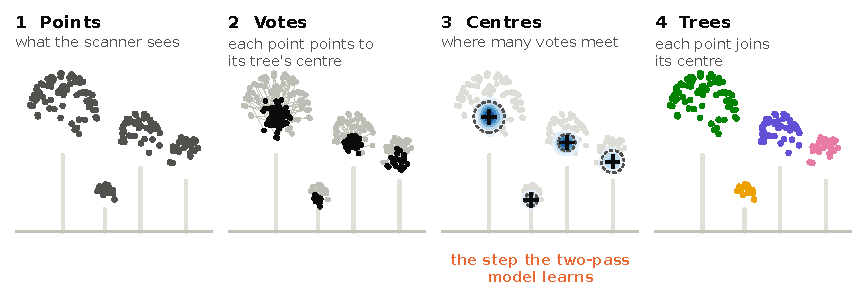
\includegraphics[width=\textwidth]{fig01_how_it_works}
\caption{How the model finds trees, shown on four made-up trees seen from the side. (1) The scanner returns points, mostly from the top of the crowns. (2) Every point votes for the centre of its tree (black dots; grey lines connect each point to its vote). (3) Tree centres (+) are where many votes meet (blue). The dashed circle is how far each tree collects votes. (4) Every point joins its tree. Step 3 is what the second pass learns.}
\label{fig:idea}
\end{figure}

\subsection{Stage 1: Model20}
\label{sec:model20}

Model20 is the production DualCrown3D network.

\paragraph{Input and backbone.} The input is the point cloud with heights above ground and the return intensity, turned into 0.25\,m voxels. The scene is processed in 20\,m $\times$ 20\,m windows with 8\,m overlap, and at most 40,000 voxels per window. A LitePT-S point transformer \citep{yue2026litept} computes a 72-number description of every voxel.

\paragraph{Two branches.}
\begin{itemize}
  \item The \emph{vote branch} predicts whether a voxel belongs to a tree and where its tree's centre is (the vote). Votes are then clustered into trees.
  \item The \emph{mask branch}, adapted from SegmentAnyTreeV2 \citep{wielgosz2026satv2}, places up to 96 queries in a window and predicts one tree mask per query. It uses a 3-layer transformer with 4 attention heads.
\end{itemize}

\paragraph{Consensus.} A rule-based step joins the two branches. Vote clusters act as anchors, masks complete them or add trees the votes missed, and remaining tree voxels are recovered locally. Every voxel gets at most one tree ID.

\paragraph{Size and training.} The network has 13.78 million parameters. It was trained on the real training plots and the HELIOS simulations. The selected checkpoint comes from a joint real and simulated fine-tuning run and was chosen on the validation plots.

\paragraph{Outputs.} Labelled LAZ files at the original point resolution and convex-hull crown polygons. Model20's outputs are in \code{output\_20\_dualcrown3d\_joint\_finetune}.

\subsection{What limits Model20}
\label{sec:bottleneck}

Before changing the architecture we measured where Model20 loses accuracy. The answer was clear. If we cluster Model20's own votes around the \emph{true} tree centres, validation point PQ rises from 0.405 to 0.670, and 523 instead of 299 of 673 trees are found. The votes already carry most of the information needed to separate trees. The weak part is deciding how many trees there are and where.

Figure~\ref{fig:votes} shows why this is hard:
\begin{itemize}
  \item Votes of one tree form a cloud around its centre, not a single point. In this example the spread is about 1\,m.
  \item Clouds of neighbouring trees touch.
  \item Small trees under a big crown have few voxels and therefore few votes.
\end{itemize}
Model20's rule-based clustering of these votes is where small trees get lost and large crowns get cut.

Three further measurements set the design of stage 2:
\begin{enumerate}
  \item Averaging Model20's votes over four rotations of the input sharpens them for free. With true centres, the averaged votes reach 0.705 instead of 0.671 point PQ.
  \item Every tree needs its own ``reach''. If each true centre may collect votes only up to the true spread of its own tree, point PQ rises to 0.744, and 132 instead of 90 of 161 small crowns are found.
  \item At 10 \vpsm, Model20's centres have recall 0.50 and precision 0.28 (1,098 instances for 624 trees). A second stage that keeps them where it is unsure keeps their errors. Stage 2 therefore \emph{replaces} them.
\end{enumerate}

\begin{figure}[t]
\centering
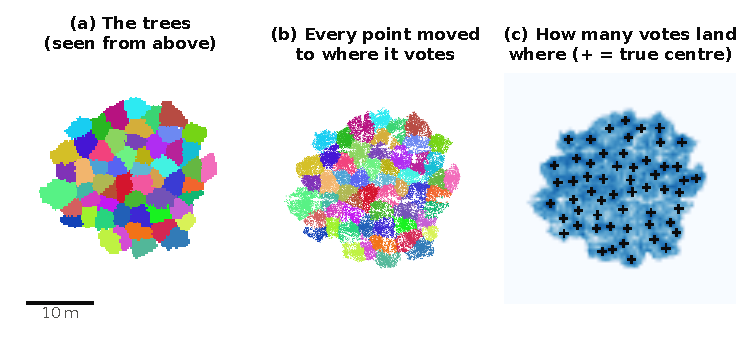
\includegraphics[width=0.88\textwidth]{fig02_votes_real_plot}
\caption{The same idea on a real plot (\col{CEDAR\_CYPRESS} Kokonoe~17, annotated trees, points above 2\,m, seen from above). (a) The trees, one colour each. (b) Every point drawn where Model20 says its tree's centre is: each tree shrinks towards its centre. (c) The number of votes per 0.5\,m cell (darker = more) and the true centres (+). The clouds of neighbouring trees touch, which is why finding the centres is hard. This plot was used for model selection; it is shown only as an illustration.}
\label{fig:votes}
\end{figure}

\subsection{Stage 2a: a detector that looks for meeting votes}
\label{sec:detector}

\paragraph{Vote volume.} For every 20\,m window we count the averaged votes in an 80 $\times$ 80 $\times$ 40 grid: 0.25\,m horizontally and 1\,m in the height of the voted centre. Each cell holds 14 channels:
\begin{itemize}
  \item how many votes arrive and how confident they are;
  \item from which direction they arrive;
  \item how much the votes disagree across the four rotations;
  \item the canopy height in that column;
  \item the point density of the window.
\end{itemize}

\paragraph{Network and outputs.} A small 3-D U-Net (three resolution levels) reads this volume. At 0.5\,m resolution it predicts three things:
\begin{itemize}
  \item a \emph{centre heat}: how likely a tree centre is in the cell;
  \item a sub-cell \emph{offset} that places the centre exactly;
  \item an \emph{extent}: how far that tree's votes reach.
\end{itemize}
For training, the target centre of a tree is the median of its own votes, not its geometric centroid. The target extent is the 90th percentile of the distance of its votes to that median. Both are measured in a space where height counts one third as much as horizontal distance, the same space in which votes are later assigned.

\paragraph{Training data.} The detector is trained on a 40/40/20 mix of the dense training plots, their thinned versions (Model20 rerun on each), and the HELIOS simulations. This exposes it to the target density during training.

\paragraph{Ensemble.} Four independently trained detectors are averaged, each evaluated on four flips of the window. Candidates are all heat peaks with a score of at least 0.1, plus every Model20 centre that no peak covers.

\subsection{Stage 2b: a verifier that checks each candidate}

A gradient-boosted tree classifier scores every candidate with 40 features that a local 3-D view cannot see. Examples:
\begin{itemize}
  \item whether a stronger candidate claims the same votes;
  \item whether the candidate sits in the middle of its voters or at their edge;
  \item how many votes only this candidate can explain;
  \item whether the candidate is a fragment of a Model20 tree.
\end{itemize}
The final score is the mean of the verifier's probability and the detector's heat. Candidates with a score of at least 0.7 become trees. Because the verifier also scores Model20's own centres, stage 2 can add, move and remove trees in one decision.

\subsection{Assignment}

Each vote goes to the centre with the smallest distance relative to that centre's reach, among the centres whose reach covers it. The reach is 1.5 times the predicted extent, kept between 1 and 4\,m. Votes that no centre reaches stay unlabelled. Model20's size filters are applied last: at least 12 voxels, 2\,m height and 0.75\,\sqm{} crown area. Each point records in the LAZ field \code{assignment\_source} whether its tree came from a kept Model20 centre (3), a stage-2 centre near a Model20 centre (8) or a new stage-2 centre (9).

\subsection{Coverage fallback}
\label{sec:fallback}

Because stage 2 replaces Model20's trees, a tree that the detector misses is left unlabelled rather than absorbed by a neighbour. On plots this mostly costs coverage, not PQ. On the real target scene, however, it leaves a third of the tree voxels without a label (Section~\ref{sec:scene}).

The optional fallback (\code{--fallback 0.7}) repairs this. A Model20 tree becomes a tree again, made of its unlabelled voxels, if stage 2 left at least 70\,\% of its voxels (and at least 12) unlabelled. Where stage 2 found trees, nothing changes. Such points carry \code{assignment\_source} = 10.

The fallback threshold was chosen on validation. There it costs about 0.01 PQ and raises the share of annotated tree voxels with a label from 83 to 95\,\% at 10 \vpsm. The fallback was \emph{not} part of the held-out test plan (Section~\ref{sec:protocol}); its independent check is the Weiser data (Section~\ref{sec:weiser}).

Figure~\ref{fig:variants} summarises how the three variants differ.

\begin{figure}[t]
\centering
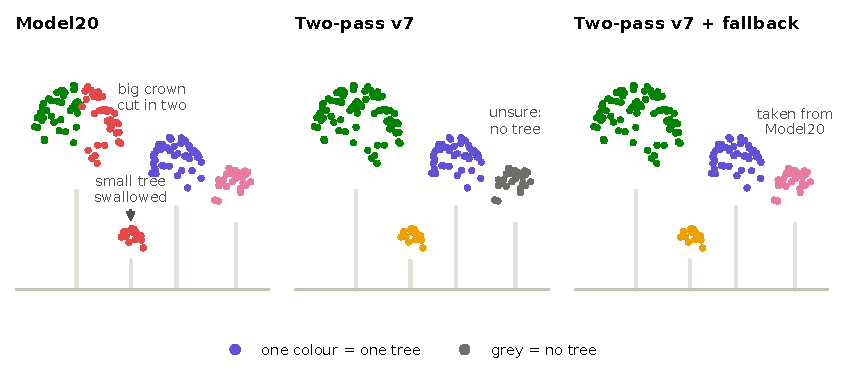
\includegraphics[width=\textwidth]{fig03_three_variants}
\caption{What the three variants typically do, on the made-up trees of Figure~\ref{fig:idea}. Model20 often cuts a large crown into two trees and lets a large tree take the votes of a small neighbour. Two-pass v7 keeps the large crown whole and finds the small tree, but drops a tree it is not sure about. With the fallback, such a tree is taken back from Model20. This is a sketch of the errors measured in Section~\ref{sec:results}, not a result.}
\label{fig:variants}
\end{figure}

\section{How we measured}
\label{sec:protocol}

\paragraph{Main metrics.} We report point and crown PQ, source-balanced across collections. Beside them we report diagnostics that the user cares about:
\begin{itemize}
  \item \emph{small crowns found}: reference crowns of at most 10\,\sqm{} that get a matching prediction;
  \item \emph{large-tree recall}: the share of reference trees with at least 500 voxels that are matched;
  \item \emph{split trees}: reference trees of which two or more predictions each hold at least 20\,\% of the voxels;
  \item \emph{merged predictions}: predictions that hold at least half of each of two or more reference trees.
\end{itemize}

\paragraph{Gates before testing.} Before the first v7 detector was trained we froze a protocol with three validation gates, all against Model20 on the same plots:
\begin{itemize}
  \item \emph{dense plots}: PQ, precision and large-tree recall no worse, and at least 16 of 161 small crowns found;
  \item \emph{plots thinned to 10 \vpsm}: point \emph{and} crown PQ at least 0.02 higher;
  \item \emph{HELIOS simulations}: PQ, precision and large-tree recall no worse.
\end{itemize}
One configuration had to pass all three.

\paragraph{Held-out test.} The test plan named the primary candidate (the ensemble with the verifier) and one secondary candidate (without the verifier) before any v7 test was run. Each test suite was then evaluated once.

\paragraph{Exposure of the test plots.} The HELIOS test plots had never been read before. The real dense and thinned test plots had been read for earlier versions (v5, v6). They are therefore a paired regression benchmark rather than a pristine hold-out.

\section{Results}
\label{sec:results}

\subsection{Held-out test}

Table~\ref{tab:heldout} and Figure~\ref{fig:heldout} give the main result. Two-pass v7 is better than Model20 on every held-out suite:
\begin{itemize}
  \item by 0.09--0.11 point PQ and 0.05--0.06 crown PQ;
  \item by 0.15--0.22 point PQ over the classical CHM pipeline, which was run with its production parameters and scored with the same code.
\end{itemize}
The gain is largest at low density. There, Model20's own clustering is weakest, and the detector was trained to cope with that density.

\begin{table}[t]
\centering\footnotesize
\caption{Held-out test results, source-balanced point / crown PQ at IoU 0.5 (higher is better). ``Annotated'' ignores predictions on unannotated vegetation. The classical pipeline was scored on the native-density plots only.}
\label{tab:heldout}
\begin{tabular}{lccccc}
\toprule
& \multicolumn{2}{c}{24 real plots, native} & \multicolumn{2}{c}{same, thinned to 10 \vpsm} & 7 HELIOS plots \\
\cmidrule(lr){2-3}\cmidrule(lr){4-5}\cmidrule(lr){6-6}
Model & point / crown & annotated & point / crown & annotated & point / crown \\
\midrule
Classical CHM pipeline & 0.292 / 0.270 & 0.370 & -- & -- & -- \\
Model20 & 0.418 / 0.422 & 0.507 & 0.389 / 0.322 & 0.466 & 0.612 / 0.576 \\
\textbf{Two-pass v7} & \textbf{0.512 / 0.486} & \textbf{0.611} & \textbf{0.500 / 0.374} & 0.578 & \textbf{0.719 / 0.638} \\
v7 without verifier & 0.496 / 0.473 & 0.603 & 0.491 / 0.356 & \textbf{0.579} & 0.716 / 0.622 \\
\midrule
\multicolumn{6}{l}{\emph{Same suites, source-balanced point F1 (for orientation, see Section~\ref{sec:literature})}}\\
Model20 & \multicolumn{2}{c}{0.519} & \multicolumn{2}{c}{0.484} & 0.767 \\
Two-pass v7 & \multicolumn{2}{c}{0.610} & \multicolumn{2}{c}{0.599} & 0.842 \\
\bottomrule
\end{tabular}
\end{table}

\begin{figure}[t]
\centering
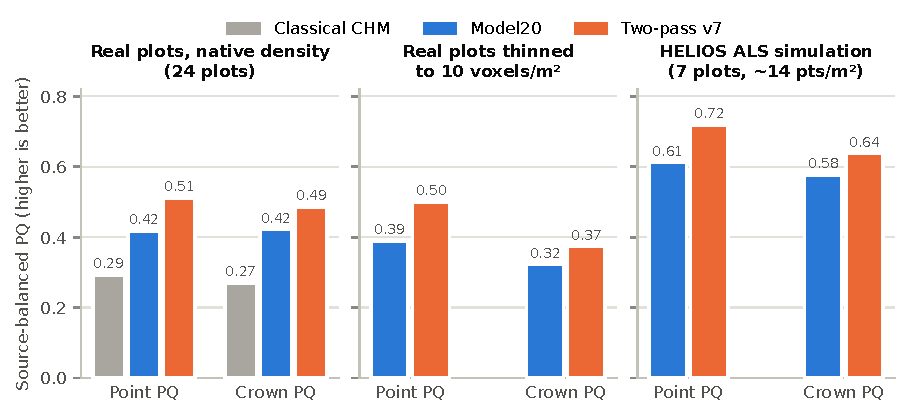
\includegraphics[width=\textwidth]{fig04_heldout_pq}
\caption{Held-out point and crown PQ in the three test suites. The classical CHM pipeline (grey) was evaluated on the native-density plots only.}
\label{fig:heldout}
\end{figure}

\subsection{What changed}

The gain is not a trade of one error for another (Figure~\ref{fig:errors}). On the native-density test plots, v7:
\begin{itemize}
  \item finds four times as many small crowns (88 against 21 of 241);
  \item finds more large trees (recall 0.79 against 0.62);
  \item halves the number of reference trees cut into pieces (72 against 140);
  \item is \emph{more} precise, not less (0.56 against 0.45 point precision).
\end{itemize}
Merged predictions also drop, from 150 to 106. The version without the verifier finds even more small crowns (95) and large trees (0.80) at lower precision (0.52). Figure~\ref{fig:test_plots} shows what this looks like on four test plots.

\begin{figure}[t]
\centering
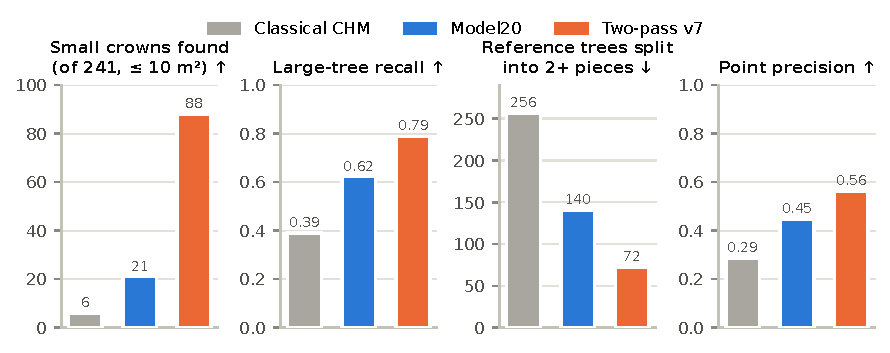
\includegraphics[width=\textwidth]{fig05_error_profile}
\caption{Error profile on the 24 native-density test plots. Arrows show which direction is better. ``Split'' counts reference trees of which at least two predictions each hold 20\,\% or more.}
\label{fig:errors}
\end{figure}

\begin{figure}[p]
\centering
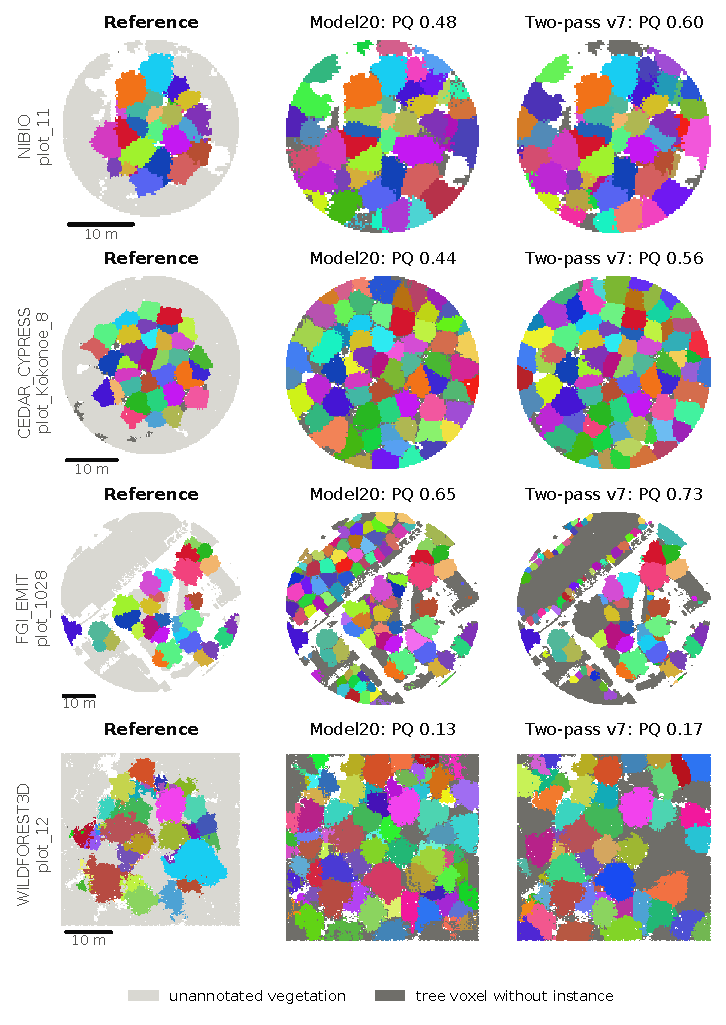
\includegraphics[width=0.86\textwidth]{fig06_test_plots}
\caption{Four held-out test plots seen from above (voxels above 2\,m). Each comes from a different collection; in each collection we show the plot whose gain from v7 is closest to that collection's median gain, so these are typical cases, not the best ones. A prediction that matches a reference tree (IoU $\geq$ 0.5) has that tree's colour. Light grey: vegetation not annotated in the reference. Dark grey: predicted tree voxels with no tree ID. Model20 cuts several \col{NIBIO} and \col{CEDAR\_CYPRESS} crowns into two; v7 joins most of them. On \col{FGI\_EMIT} and \col{WILDFOREST3D}, v7 leaves large areas of unannotated vegetation without a tree, which the PQ does not penalise but a map user would notice (Section~\ref{sec:fallback}). \col{WILDFOREST3D}, with wide and diffuse crowns, remains the weakest collection for both models.}
\label{fig:test_plots}
\end{figure}

\subsection{Consistency}

The gain is consistent across collections and plots:
\begin{itemize}
  \item Point PQ rises in every collection at both densities (Figure~\ref{fig:collections}), most in \col{NIBIO}, \col{FGI\_EMIT} and \col{CEDAR\_CYPRESS}.
  \item Per plot, v7 is better on 23 of 24 native-density plots, 24 of 24 thinned plots and all 7 HELIOS plots (Figure~\ref{fig:per_plot}). The one exception (\col{WILDFOREST3D} plot~28) is a tie: 0.253 against 0.249.
  \item Crown PQ is less uniform. It is flat on \col{CULS} and \col{WILDFOREST3D} at native density and falls on \col{NIBIO} when thinned (0.330 to 0.302), although point PQ rises there.
\end{itemize}

\begin{figure}[t]
\centering
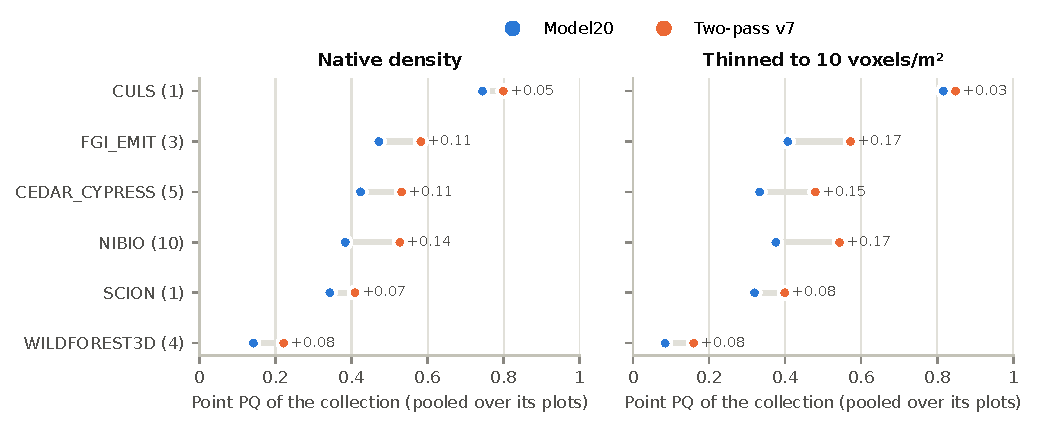
\includegraphics[width=\textwidth]{fig07_per_collection}
\caption{Point PQ per collection, pooled over its test plots (number of plots in brackets), for Model20 (blue) and two-pass v7 (orange).}
\label{fig:collections}
\end{figure}

\begin{figure}[t]
\centering
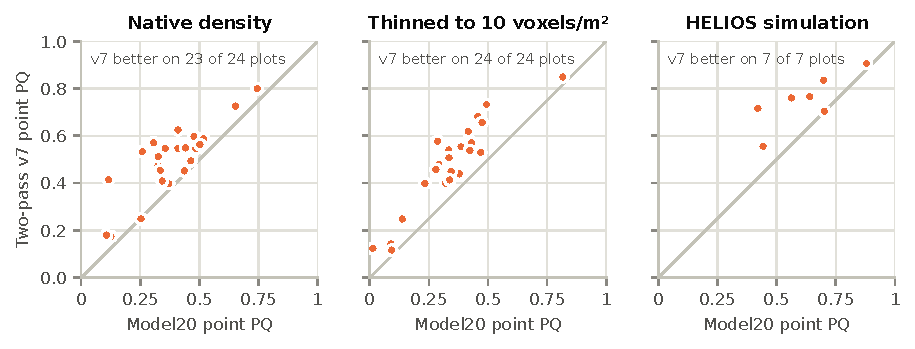
\includegraphics[width=\textwidth]{fig08_per_plot}
\caption{Point PQ of every test plot, Model20 against v7. Points above the diagonal are plots where v7 is better.}
\label{fig:per_plot}
\end{figure}

\subsection{Density}

On validation, Model20's crown PQ falls from 0.44 at native density to 0.31 at 10 \vpsm. Two-pass v7 keeps a lead of 0.05--0.10 in both point and crown PQ at 10, 25 and native density (Figure~\ref{fig:density}).

\begin{figure}[t]
\centering
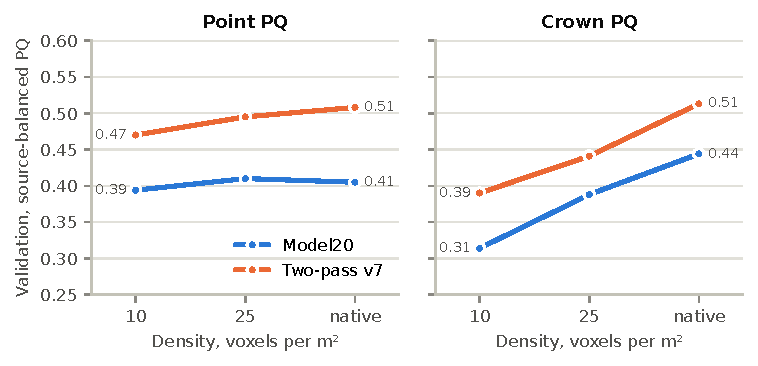
\includegraphics[width=0.72\textwidth]{fig09_density_validation}
\caption{Validation PQ on the same 14 plots at three densities. These numbers were used for model selection and are therefore optimistic; Table~\ref{tab:heldout} gives the held-out numbers.}
\label{fig:density}
\end{figure}

\subsection{Where the gain comes from}

Table~\ref{tab:buildup} shows how the gain was built up on validation. Three findings:
\begin{itemize}
  \item A single detector already gives most of the gain.
  \item Longer training and averaging four detectors add a little. The detector is saturated: seeds, wider networks, size-adaptive targets and other density mixes all land within about 0.02 of each other.
  \item The verifier buys precision and costs some small crowns. This is why the version without it is kept as a secondary operating point.
\end{itemize}

\begin{table}[t]
\centering\small
\caption{How the gain was built up on validation. ``Gain'' is the selection measure: the summed improvement over Model20 in $\sqrt{\text{point PQ} \times \text{crown PQ}}$ on dense and thinned validation. Small crowns: of 161 on dense validation.}
\label{tab:buildup}
\begin{tabularx}{\textwidth}{Lcccc}
\toprule
Step & Gain & Dense: point / crown & Thinned: point / crown & Small crowns, dense \\
\midrule
Model20 & 0 & 0.405 / 0.444 & 0.394 / 0.314 & 6 \\
earlier two-pass v5 & 0.02 & 0.416 / 0.446 & 0.404 / 0.333 & 18 \\
one detector, 40--50 epochs (3 seeds) & 0.10--0.12 & 0.46--0.49 / 0.47--0.49 & 0.45--0.46 / 0.37--0.38 & 40--56 \\
one detector, 120 epochs & 0.13 & 0.479 / 0.491 & 0.467 / 0.387 & 49 \\
four detectors averaged & 0.147 & 0.494 / 0.496 & 0.468 / 0.390 & 46 \\
+ verifier (final) & \textbf{0.163} & \textbf{0.508 / 0.513} & \textbf{0.470 / 0.390} & 34 \\
\bottomrule
\end{tabularx}
\end{table}

\subsection{Real sparse ALS: the Weiser plots}
\label{sec:weiser}

The test plots above are either dense, thinned or simulated. The closest we have to labelled real sparse ALS is the ALS of \citet{weiser2022}. It covers 12 scans from German forests with 1,476 reference trees whose segments were checked by hand, thinned from their native 72 \ppsm{} to 14 \ppsm. None of these scans was used to train or select any of the models. They were scored with the error breakdown of our trunk-reconstruction project (Figure~\ref{fig:weiser}).

\begin{figure}[t]
\centering
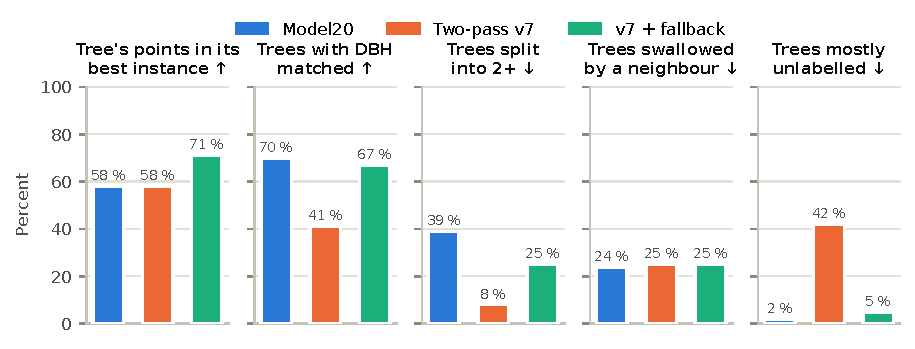
\includegraphics[width=\textwidth]{fig10_weiser_real_als}
\caption{Real ALS from \citet{weiser2022}, 12 scans thinned to 14 \ppsm, 1,476 reference trees (points above 2\,m). ``Tree's points in its best instance'' is the median share of a reference tree's points that fall in the prediction holding most of them. ``Trees with DBH matched'' is the share of reference trees with a measured stem diameter that get an instance. Source: \code{trunk\_reconstruction/reports/SEGMENTATION.md}.}
\label{fig:weiser}
\end{figure}

\paragraph{v7 alone.} It nearly eliminates split trees (39\,\% to 8\,\%). But it leaves 42\,\% of the trees mostly unlabelled, so only 41\,\% of the trees with a stem measurement get an instance. The cause is the 4\,m reach cap: the votes of very tall trees (on one plot, 45--50\,m Douglas firs) scatter further than 4\,m from their centre.

\paragraph{v7 with the fallback.} It restores coverage (5\,\% unlabelled, 67\,\% matched against Model20's 70\,\%) and keeps more of each tree together:
\begin{itemize}
  \item the median share of a tree's points in its best instance rises from 58 to 71\,\%;
  \item fewer trees are split (25\,\% against 39\,\%).
\end{itemize}
In the downstream trunk model, this gives a significantly better stem diameter (DBH) on the trees found by both: the 95\,\% plot-bootstrap interval of the difference to Model20 is $-1.3$ to $-0.4$\,cm.

\paragraph{What neither fixes.} Trees swallowed by a neighbour stay at 24--25\,\% in all three variants. Stage 2 works on Model20's votes, and the points of a swallowed tree vote with their host.

\subsection{The reference scene}
\label{sec:scene}

The target scene has no labels, so only counts and pictures can be compared (Table~\ref{tab:scene}, Figure~\ref{fig:scene}).

\paragraph{v7 alone is much quieter here than on the test plots.} It keeps 4,143 trees where Model20 has 9,644, and a third of the predicted tree voxels end up without a tree (10\,\% for Model20). On thinned validation the same model left only 17\,\% unlabelled. Thinned drone plots and HELIOS simulations therefore do not fully represent this scan.

\paragraph{With the fallback.} Stage 2 trees and Model20 trees are combined: 4,143 from stage 2 and 4,188 kept from Model20. Every tree voxel that Model20 labels is labelled again. In the window of Figure~\ref{fig:scene}, the largest grey areas of v7 alone lie in the tall stand on the right, in line with the Weiser finding about large crowns.

\begin{table}[t]
\centering\small
\caption{Reference scene, four 500\,m core tiles (no ground truth).}
\label{tab:scene}
\begin{tabular}{lcccc}
\toprule
& Model20 & Two-pass v7 & v7 + fallback & Classical CHM \\
\midrule
Trees & 9,644 & 4,143 & 8,331 & 6,688 \\
Voxels with a tree ID & 1.62 M & 1.16 M & 1.62 M & -- \\
Crowns $\leq$ 10\,\sqm & 1,948 & 1,023 & 2,506 & -- \\
Median crown area & 15.5\,\sqm & 20.1\,\sqm & 14.0\,\sqm & 16.6--29.0\,\sqm{} per tile \\
Output folder & \code{output\_20} & \code{output\_38} & \code{output\_39} & \code{segmentatiion\_benchmark} \\
\bottomrule
\end{tabular}
\end{table}

\begin{figure}[p]
\centering
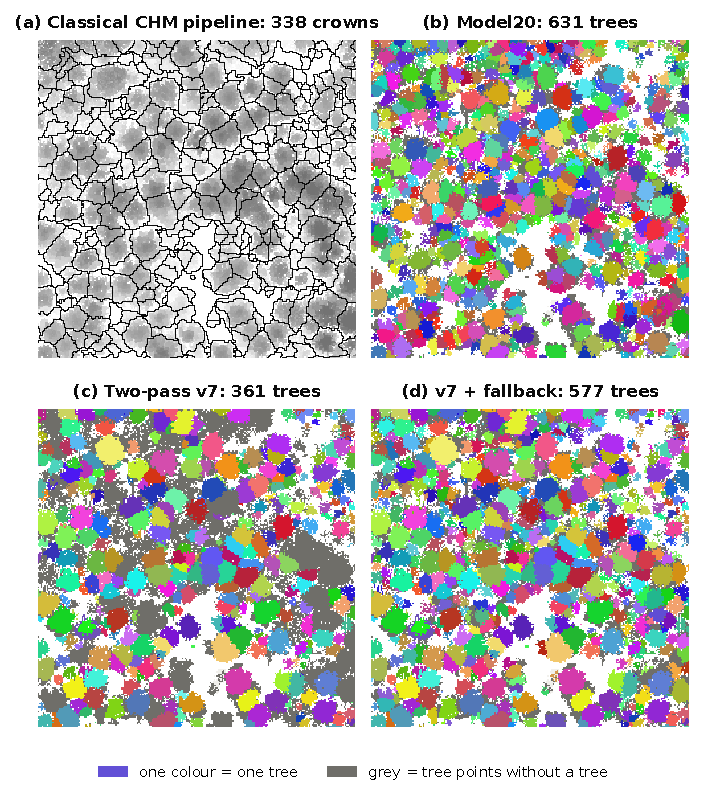
\includegraphics[width=0.8\textwidth]{fig11_reference_scene}
\caption{A 120\,m $\times$ 120\,m part of tile 764000\_197000 of the reference scene (lower-left corner at x = 764,280, y = 197,260, EPSG:2180), seen from above. (a) Crowns of the classical production pipeline over the canopy height (darker = taller). (b)--(d) Trees of the three deep variants; counts include trees that only partly lie in the window. Dark grey: points the model calls tree but gives no tree. Two-pass v7 alone (c) leaves large grey areas; the fallback (d) fills them with Model20 trees.}
\label{fig:scene}
\end{figure}

\subsection{Cost}

Two-pass v7 is slower than Model20 (Table~\ref{tab:cost}):
\begin{itemize}
  \item Stage 1 runs four more times for the rotation ensemble.
  \item Stage 2 runs four detectors on four flips each.
\end{itemize}
On the test plots the full pipeline takes about 4 (native density) to 8 (thinned) times as long as Model20. One 120-epoch detector instead of four would cut stage-2 time to a quarter for a loss of about 0.013 in the selection gain.

Training takes 20--50 minutes per detector on one A100 and about 20 minutes for the verifier.

\begin{table}[t]
\centering\small
\caption{Running time in seconds. Laptop GPU: NVIDIA RTX PRO 500 (6\,GB); A100: Cyfronet Athena.}
\label{tab:cost}
\begin{tabularx}{\textwidth}{L*{4}{>{\centering\arraybackslash}p{2.1cm}}}
\toprule
& Stage-1 forward & Stage-1 consensus & Vote ensemble (4 rotations) & Stage 2 \\
\midrule
24 test plots, native, laptop & 46 & 27 & 113 & 97 \\
24 test plots, thinned, laptop & 14 & 2 & 46 & 60 \\
Reference scene, 78\,ha, 7.7 M voxels & 228 & 17 & 963 (laptop) & 360 (A100) \\
\bottomrule
\end{tabularx}
\end{table}

\section{Comparison with other methods}
\label{sec:literature}

\subsection{Same plots, same code: the classical pipeline}

The only method we have scored with exactly our protocol is the classical CHM pipeline. We ran it with its production parameters on the plot CHMs; our runner reproduces the production script's polygons exactly on all 38 validation and test plots. On the 24 test plots it reaches 0.292 / 0.270 point / crown PQ. That is 0.13 below Model20 and 0.22 below v7. It finds 6 of 241 small crowns and splits 256 reference trees.

Two caveats favour the deep models:
\begin{itemize}
  \item the plot CHMs are raw maximum-height rasters with gaps, not the production CHM product;
  \item the plots are smaller than the 25\,m buffer the production pipeline uses.
\end{itemize}
The size of the gap and the error profile (Figure~\ref{fig:errors}) agree with published comparisons: deep models beat watershed on thinned ALS at all densities \citep{ruoppa2025fgiemit,wielgosz2024sat}. On the reference scene the classical pipeline produces 6,688 crowns, between v7 alone and v7 with the fallback.

\subsection{Published deep-learning methods}

Table~\ref{tab:literature} collects published results as their authors report them. Our own numbers are in the last rows.

\begin{table}[p]
\centering\footnotesize
\caption{Published tree instance segmentation methods, results as reported by their authors (state of October 2026). F1, precision (P), recall (R) and coverage (Cov) in \%. \textbf{The rows use different data and metrics and must not be ranked against each other or against our PQ values}; see the text.}
\label{tab:literature}
\begin{tabularx}{\textwidth}{>{\raggedright\arraybackslash}p{2.9cm}>{\raggedright\arraybackslash}p{1.9cm}LL>{\raggedright\arraybackslash}p{1.8cm}}
\toprule
Method & Venue & Reported result & Evidence at ALS density & Code / weights \\
\midrule
SegmentAnyTreeV2 \citep{wielgosz2026satv2}: PTv3 backbone + mask decoder & arXiv 2026 & FOR-instanceV2 test: F1 85.0 (P 90.5, R 80.2), Cov 90.7 & trained on 10--50,000 \ppsm; no real sparse ALS test & not found \\
ForPT \citep{yue2026forpt}: LitePT foundation model, pretrained mostly on ALS & arXiv 2026 & FOR-instanceV2: F1 84.7 fine-tuned (85.5 trained from scratch) & pretraining data about 200 \ppsm{} on average & repository announced \\
ForestMamba \citep{nguyen2026forestmamba}: queries seeded at CHM peaks & BMVC 2026 & FOR-instanceV2: F1 83.4 (ForestFormer3D 82.3 in the same evaluation) & dense data only & yes \\
ForestFormer3D \citep{xiang2025ff3d} & ICCV 2025 & FOR-instanceV2: F1 82.8, Cov 81.2; FGI-EMIT: F1 73.3, best of the methods tested there & ahead of unsupervised methods down to 10 \ppsm{} (thinned), recall falls with density & yes, with weights \\
ForAINet \citep{xiang2024forainet} & RSE 2024 & FOR-instance (v1): F1 85.1; FOR-instanceV2: 70.8--72.4 (reported by ForestFormer3D) & ULS 500--9,500 \ppsm & yes \\
SegmentAnyTree \citep{wielgosz2024sat} & RSE 2024 & FGI-EMIT: F1 63.8 & FOR-instance thinned to 10 \ppsm: 58.7\,\% of trees detected (CHM-based YOLOv5: 50.5\,\%) & yes, Docker \\
Weakly supervised ALS \citep{destouches2025weak} & arXiv 2025 & detection 63.4 $\to$ 85.2\,\% after 9 pseudo-label rounds & \emph{real} ALS, 38 \ppsm & no \\
TreeLearn \citep{henrich2024treelearn} & Ecol.\ Inform.\ 2024 & FOR-instanceV2: F1 50.6 (reported by ForestFormer3D) & struggles where stems have few points & yes \\
Classical: watershed, Treeiso, AMS3D & \citet{ruoppa2025fgiemit}, \citet{cao2023} & FGI-EMIT: watershed F1 48.4, Treeiso 52.7 & real ALS, 6 pulses/m$^2$: best method (AMS3D) P 50 / R 41 even for trees over 25\,m & various \\
\midrule
\textbf{DualCrown3D Model20} (ours) & this report & 24 mixed real plots: point PQ 41.8, point F1 51.9 & thinned to 10 \vpsm: PQ 38.9; HELIOS 14 \ppsm: PQ 61.2, F1 76.7 & internal \\
\textbf{Two-pass v7} (ours) & this report & 24 mixed real plots: point PQ 51.2, point F1 61.0 & thinned: PQ 50.0; HELIOS: PQ 71.9, F1 84.2; real Weiser ALS at 14 \ppsm: Figure~\ref{fig:weiser} & internal \\
\bottomrule
\end{tabularx}
\end{table}

\paragraph{Why the numbers cannot be compared directly.}
\begin{enumerate}
  \item \textbf{Different plots.} FOR-instanceV2 has its own test split. Our 12 FOR-instance test plots are a mix of 8 plots from FOR-instance's official development split and 4 from its test split, and our other 12 test plots come from collections FOR-instanceV2 does not contain. On our 12 FOR-instance plots, pooled point F1 is 0.50 for Model20 and 0.63 for v7. This number is not comparable with published FOR-instance results, for the reasons below.
  \item \textbf{A stricter protocol.} Our main metric counts a prediction on unannotated vegetation as a false positive. About half of every real plot is unannotated, so precision and F1 are pulled down. The annotated-area PQ in Table~\ref{tab:heldout} removes part of this effect.
  \item \textbf{Different metrics.} Most papers report F1 at IoU 0.5. We select on PQ, which multiplies F1 by the mean IoU of the matches and is therefore always lower. We list our F1 for orientation.
  \item \textbf{Different density.} Published FOR-instanceV2 results are on dense drone and terrestrial scans. Our model was selected for 10--14 \ppsm, where all methods lose accuracy.
  \item \textbf{Voxels.} We evaluate on 0.25\,m voxels, not on raw points.
\end{enumerate}

\paragraph{What we can say.} Published evidence and our results point the same way in four respects.
\begin{itemize}
  \item \emph{Deep models beat classical CHM segmentation at ALS density.} On FGI-EMIT, ForestFormer3D reaches F1 73.3 against 48.4 for watershed; on our plots, v7 reaches 0.51 PQ against 0.29.
  \item \emph{Small and suppressed trees are the hardest part for everyone.} On FGI-EMIT, even the best model finds 39.7\,\% of under-dominant trees \citep{ruoppa2025fgiemit}. In our test, crowns of 4\,\sqm{} or less remain almost undetected (5 of 65).
  \item \emph{Deciding where trees are is the bottleneck.} TreeisoNet's ALS accuracy rises from 0.59 to 0.80 mIoU when its tree centres are corrected by hand.\footnote{TreeisoNet, ISPRS Open Journal of Photogrammetry and Remote Sensing, 2025, doi:10.1016/j.ophoto.2025.100083.} This mirrors our true-centre experiment (0.405 $\to$ 0.670 PQ) and is the motivation for our second pass.
  \item \emph{We found no published deep-learning tree segmenter evaluated on real ALS at 10--20 \ppsm{} with accurate tree labels.} This includes our own work: the Weiser check is real ALS, but thinned rather than natively sparse.
\end{itemize}

\paragraph{How the designs differ.} The strongest published models (SegmentAnyTreeV2, ForestFormer3D, ForestMamba) are single-pass query-and-mask models trained and evaluated on dense data. Model20's mask branch borrows from SegmentAnyTreeV2. The two-pass idea is independent of the backbone: any model that predicts per-point centre votes can be given the same second stage.

\paragraph{The missing comparison.} We have not run ForestFormer3D or SegmentAnyTree on our plots. Both have public code and weights. Running them on our 24 test plots, their thinned versions and the HELIOS plots, scored with our code, would answer where we stand. It is the first item in Section~\ref{sec:next}.

\section{Which model to use}

Table~\ref{tab:usage} summarises our recommendation.

\begin{table}[t]
\centering\small
\caption{Which variant to use.}
\label{tab:usage}
\begin{tabularx}{\textwidth}{>{\raggedright\arraybackslash}p{4.2cm}>{\raggedright\arraybackslash}p{3.2cm}L}
\toprule
Need & Variant & Why \\
\midrule
Production maps today & \textbf{Model20} (\code{output\_20}) & labels every tree voxel, validated workflow and exports; known weaknesses: small trees and split crowns \\
A complete map with fewer split crowns & \textbf{v7 + fallback} (\code{--fallback 0.7}, \code{output\_39}) & stage-2 quality where it is confident, Model20 elsewhere; on real Weiser ALS: coverage like Model20, fewer split trees, better DBH \\
Highest precision on plots, gaps acceptable & v7 primary (\code{output\_38}) & best held-out PQ; leaves trees unlabelled on real sparse scans \\
Most small crowns & v7 without verifier (run \code{ens4\_b\_detector}) & 95 of 241 small crowns, large-tree recall 0.80, lower precision \\
\bottomrule
\end{tabularx}
\end{table}

\paragraph{Why v7 is not promoted yet.} v7 improves every headline metric on three held-out suites, but three things are open:
\begin{enumerate}
  \item its accuracy on the target domain is unmeasured;
  \item it fails without the fallback on real sparse scans;
  \item the fallback was validated on validation plots and on the Weiser scans, but not on the held-out test plots.
\end{enumerate}
Until labelled data from the target region exist, the fallback variant is the safer of the two-pass options.

\section{Limitations}

\begin{itemize}
  \item \textbf{Validation was reused heavily}, including for thresholds and ensemble members. The margins are large (0.10 point PQ dense, 0.08 thinned), but the validation numbers are optimistic.
  \item \textbf{The real test plots had been read before} (for v5 and v6). Only the HELIOS test plots were fresh.
  \item \textbf{Thinning and simulation are proxies.} Neither reproduces real sparse ALS exactly. The reference scene shows this: stage 2 is much quieter there than on any proxy.
  \item \textbf{Half of each real plot is unannotated}, which caps crown PQ on real plots near 0.53 and depresses precision.
  \item \textbf{The verifier was trained on candidates of detectors that had seen the same plots.} Out-of-fold candidates were not produced.
  \item \textbf{The reach of a tree is capped at 4\,m.} Very large crowns (over about 40\,m in height) fall outside it, as the Weiser plots show.
  \item \textbf{Swallowed trees are untouched.} Stage 2 cannot separate a tree whose points vote with a neighbour.
  \item \textbf{Very small crowns} ($\leq$ 4\,\sqm) remain almost undetected. Wide, diffuse crowns (\col{WILDFOREST3D}) remain weak (point PQ 0.22).
  \item \textbf{Cost:} 4--8 times Model20's running time on the test plots.
  \item \textbf{Crown polygons are convex hulls}, as in Model20's exporter.
\end{itemize}

\section{Next steps}
\label{sec:next}

\begin{enumerate}
  \item \textbf{Compare with ForestFormer3D and SegmentAnyTree under our protocol}, using their public weights on our test suites.
  \item \textbf{Label 2--3\,ha of the target scene.} This is the single most valuable step: it would allow thresholds, the fallback and stage 2 itself to be judged where they will be used.
  \item \textbf{Raise the reach cap for tall trees.} An 8\,m cap with a detector trained on tall-stand data is in preparation.
  \item \textbf{Produce out-of-fold candidates for the verifier}, to remove the in-sample caveat.
  \item \textbf{Improve the votes themselves}, by retraining stage 1 with a larger budget. Better votes help detection, assignment and swallowed trees at once.
  \item \textbf{Reduce cost} by distilling the four detectors into one and dropping the flip averaging.
\end{enumerate}

\appendix
\section{Reproduction}

All paths are relative to \code{DL\_model\_version}. Python environment: \code{.venv-gpu}.

\begin{itemize}
  \item \textbf{Stage 1 (Model20)} checkpoint:\\ \code{outputs/dualcrown3d\_joint\_campaign\_v1/runs/repeat\_20260930/weights/best.pt}\\ (SHA-256 \code{e0ffb413\ldots 6688}).
  \item \textbf{Stage 2} ensemble with verifier:\\ \code{outputs/dualcrown3d\_two\_pass\_v1/runs/ens4\_b/weights/best.pt}\\ (SHA-256 \code{3108fe6c\ldots 75aa}), configuration \code{mean\_heat\_t0.7\_nms0\_extent1.5\_norm}.
  \item \textbf{Frozen protocol and test plan:}\\ \code{outputs/dualcrown3d\_two\_pass\_v1/protocol\_v7.json}, \code{test\_plan\_v7.json}.
  \item \textbf{Held-out results:} \code{output\_32} to \code{output\_37},\\ each with \code{comparison.json} and \code{comparison.xlsx}. Reference scene: \code{output\_38} and \code{output\_39}. Classical baseline:\\ \code{outputs/classical\_chm\_baseline\_v1}.
  \item \textbf{Full engineering report:} \code{reports/two\_pass\_v7\_vote\_field.md}.
  \item \textbf{Figures:} \code{reports/technical\_paper/make\_figures.py} regenerates all figures of this report from the files above.
\end{itemize}

\begin{small}
\begin{verbatim}
# held-out suite (dense | thinned | helios) and reference scene
.venv-gpu/bin/python scripts/evaluate_vote_field_test.py --run ens4_b \
    --suite dense --output <new folder>
.venv-gpu/bin/python scripts/predict_vote_field_scene.py --run ens4_b \
    --output-dir <new folder> --fallback 0.7
# figures of this report
.venv-gpu/bin/python reports/technical_paper/make_figures.py
\end{verbatim}
\end{small}

\section{What did not help}

\begin{table}[h]
\centering\small
\begin{tabularx}{\textwidth}{>{\raggedright\arraybackslash}p{5.6cm}L}
\toprule
Idea & Outcome \\
\midrule
Second pass that generates new masks on frozen features & worse than Model20 in three variants \\
Keeping Model20's centres where stage 2 is unsure (v5/v6) & no gain at 10 \vpsm; replacing them is better once the detector is good \\
Model20's instance embedding as an extra cue & lowers the true-centre ceiling (0.761 $\to$ 0.699) \\
Size-adaptive heat targets & no gain on the selection measure \\
Growing crowns into unlabelled neighbouring voxels & more coverage, lower PQ \\
Learned voxel-to-centre assignment (stage 3) & parity with the geometric rule (79\,\% correct slot), although its ceiling is 0.93 PQ \\
Larger query decoder with superpoints (Model22) & more small trees, heavy over-segmentation \\
\bottomrule
\end{tabularx}
\end{table}

\bibliographystyle{plainnat}
\bibliography{references}

\end{document}
